% Report/chapters/1d.tex
\hspace{5mm}In this chapter, we will consider the following boundary value problem for the poisson equation and demonstrate how the Finite Element Method can be implmented in MATLAB to compute the solutions to different Ordinary Differential Equations subjected to \textbf{Dirichlet, Neumann and Robin} Boundary Conditions.
\section{Weak formulation}
\hspace{5.4mm}Consider the \emph{2-Point Boundary Value Problem} in 1D,
\begin{eqnarray}
-u''(x) &=& f(x) \quad \text{in} \quad \Omega \equiv (0,1)\label{model}\\
u(0) &=& u(1) \ \ = \ \ 0
\end{eqnarray}
Now, let us look at the general procedure that is usually followed to find out the \textbf{Finite Element Solution} of the problem.

\begin{enumerate}
	\item \textbf{Derive the Variational/Weak Formulation}:
	We shall now give an abstract formulation of the finite element method for elliptic problems. This makes it possible to give a unified treatment of many problemsin mathematics and physics. Considering the Galerkin Approach, we construct the weak formulation of our \textbf{2-Point BVP} by multiplying both sides of \ref{model} with a \textbf{test function} $v$ satisfying $v(0) = v(1) = 0$ and integrating it over the domain $\Omega \equiv (0,1)$ .
	\begin{equation}
	-\int_{0}^{1} u'' v\ dx = \int_{0} ^{1} fv \ dx
	\end{equation}
	\begin{equation}
	- \ u'v \ \Big|_0^1 + \int_{0}^{1} u'v' \ dx = \int_{0}^{1} f v \ dx
	\end{equation}
	As we have assumed our test function space to follow $v(0) = v(1) = 0$, we have,
	\begin{equation}
	\int_{0}^{1} u'v' \ dx = \int_{0}^{1} f v \ dx \label{weak1}
	\end{equation}
	Equation \ref{weak1} is known as the \textbf{Weak formulation} of the problem.
	
	\item \textbf{Discretization of the problem:} For a 1D Problem, the domain is discretized into $n$ subintervals $\left[x_{i-1}, x_i\right]$ of equal length, where 
	\begin{equation}
	h = 1/n, \qquad x_i = ih, \qquad i = 1,2, \dots, n
	\end{equation}
	We should keep in mind that equal subintervals have been considered only for simplicity sake but, FEM is perfectly capable of handling an unstructured discretization.
	\item \textbf{Construct the basis functions on Master element: } Next we choose the set of basis functions depending on the problem. Let us denote them as,
	\begin{equation}
	\{\phi_i \}_{i=1,2, \dots, n}
	\end{equation}
	More about basis functions are discussed in the following sections.
	
	\item \textbf{Construct the system of equations}
	First, write down the approximate \emph{Finite Element Solution} $u_h(x)$ as a linear combination of the basis functions $\phi_i$,
	\begin{equation}
	u_h(x) = \sum_{i=1}^{n} \xi_i \phi_i(x)
	\end{equation}
	Using this in the weak formulation \ref{weak1}, we have,
	\begin{eqnarray}
	\int_{0}^{1} u'_hv' \ dx &=& \int_{0}^{1}  \bigg(\sum_{i=1}^{n} \xi_i \phi_i'\bigg) v' \ dx \label{weak2}\\	
	&=& \sum_{i=1}^{n} \xi_i \int_{0}^{1} \phi_i' v' \ dx = \int_{0}^{1} f v \ dx \label{eq2}
	\end{eqnarray}
	Now substituting $v = \phi_j, \; j=1,2,\dots, n $ in \ref{eq2}, we have a system of linear equations,
	\begin{eqnarray}
	[A]\{\xi\} &=& \{b\} \label{sys} \\ 
	A_{ij} &=& \int_{0}^{1} \phi'_i\phi'_j \ dx\\
	b_j &=& \int_{0}^{1} f\phi_j dx
	\end{eqnarray}
	
	\item \textbf{Solve the system} \ref{sys} to obtain $\xi_i$ and get $u_h(x) = \sum_{i=1}^{n} \xi_i \phi_i(x)$
	
	\item Proceed to carry out the \textbf{error analysis}.
\end{enumerate}



\subsection{Analysis of FEM}


For analysis, we consider the 1D equivalent of the model problem,
\begin{eqnarray}\nonumber
a(u,v) &:=& \int_{0}^{1} u' v'  \ dx\\ &=& \int_{0}^{1} fv \ dx \quad := \quad(f,v)
\end{eqnarray}

Next we present some of the interesting properties of the \textbf{abstract form} \ref{abs}
\begin{enumerate}
	\item $a(u,v)$ is symmetric. $a(u,v) = a(v,u)$
	\item $a(u,v)$ is continuous/bounded, i.e, there exists a constant $\gamma>0$, such that
	\begin{equation}\nonumber
	|a(v,w)| \le \gamma \lVert v\rVert_V \lVert w \rVert_V \quad \forall v,w \in V
	\end{equation}
	\item $a(u,v) $ is coercive/V-Elliptic, i.e, there exists a constant $\alpha > 0$, such that
	\begin{equation}
	a(v,v) \ge \alpha \lVert v \rVert_V^2 \quad \forall v\in V
	\end{equation}
	\item $(f,v)$ is bounded. i.e, there exists a constant $\Lambda > 0$ such that
	\begin{equation}
	|(f,v)| \le \Lambda \lVert v \rVert_V \quad \forall v \in V
	\end{equation}	
\end{enumerate}
An important consequence of the properties is the \textbf{uniqueness} of the solution to the variational problem which is given by the \textbf{Lax-Milgram Theorem}. Now that we have addressed the issue of uniqueness of the solution, we now look at the basis functions for the model problem.\\

Since the space $V = H^1_0(\Omega)$ is an infinite dimensional space, searching for the finite element solution is an impossible task for the computer. So we ``approximate" the Infinite Dimensional space by a Finite Dimensional space $V_h \subset V$. Let,
\begin{equation}\nonumber
V_h = span\{\phi_1, \phi_2, \dots, \phi_n\}
\end{equation}
where $\phi_i$ are the basis functions for the finite dimensional space $V_h$. Hence any function in $V_h$ can be represented as,
\begin{equation}\nonumber
v_h(x) = \sum_{i=1}^{n} \xi_i \phi_i(x)
\end{equation}
\pagebreak
\subsection{Basis functions}
A common choice for the basis functions for our \textbf{Model Problem in 1D} are the linear Lagrange basis functions/Hat functions.
\begin{figure}[h]
	\centering
	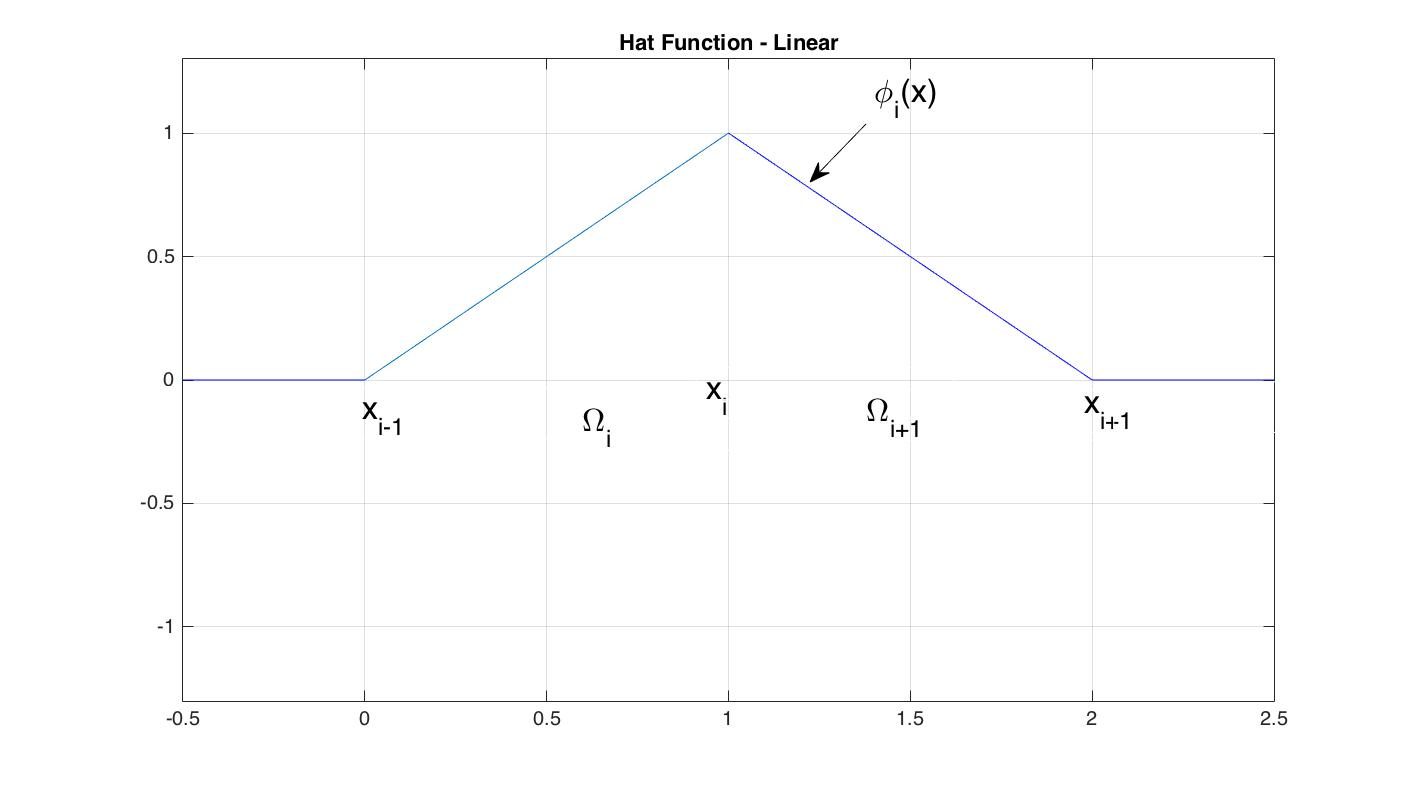
\includegraphics[width=12cm,height=8cm]{images/hat.jpg}
	\caption{Hat Function}
\end{figure}
\begin{equation}
\phi_i(x) = \left\{
\begin{array}{ll}
\frac{x-x_{i-1}}{h} & x_{i-1}\leq x\leq x_i \\
\frac{x_{i+1}-x}{h} & x_i\leq x\leq x_{i+1} \\
0 & otherwise\\
\end{array} 
\right. \label{basis1d}
\end{equation}
Observe that  
\begin{eqnarray}
\phi_i(x_j) &=& \delta_{ij}, \quad \text{where} \label{kd}\\
\delta_{ij} &=& \left\{ 
\begin{array}{ll}
1, & i=j\\
0, & i\ne j	
\end{array}
\right.
\end{eqnarray}
at nodes $x_j$. The expresssion \ref{basis1d} can be obtained by assuming a linear equation of the form $\phi_i(x) = a+b\ x$ and using the Kronecker Delta Property \ref{kd}. The function defined above is said to have a \textbf{Compact Support} in $\Omega$ which means that the function is non-zero only at certain points in the domain. This property is reflected in the \textbf{sparse nature} of the Global Stiffness Matrix.\\

To find out the solution at each nodes in the domain, we construct stiffness matrix $K^e$ and load vector $f^e$ at the element level and then assemble them to obtain the global system and solve it. So at the element level, we have the system of equations
\begin{eqnarray}
[K^e] \{u^e\} = \{f^e\}
\end{eqnarray}
The local numbering of the linear basis functions in an element $\Omega^e$ is shown in Figure 1.2(a). Let $\psi^e_1 \ \text{and} \ \psi^e_2$ be the basis function in an element $\Omega^e$. If the element size is $h_e$, then for the model problem in 1D, we have,
\begin{equation}
K^e = \Bigg[\int_{0}^{h_e} \psi_i'^e \psi_j'^e \ dx \Bigg]_{i,j=1,2} = 
\begin{bmatrix}
\frac{1}{h_e} & -\frac{1}{h_e} \\\\
-\frac{1}{h_e} & \frac{1}{h_e}
\end{bmatrix}
\end{equation}
\begin{center}
	\begin{figure}[h]
		\centering
		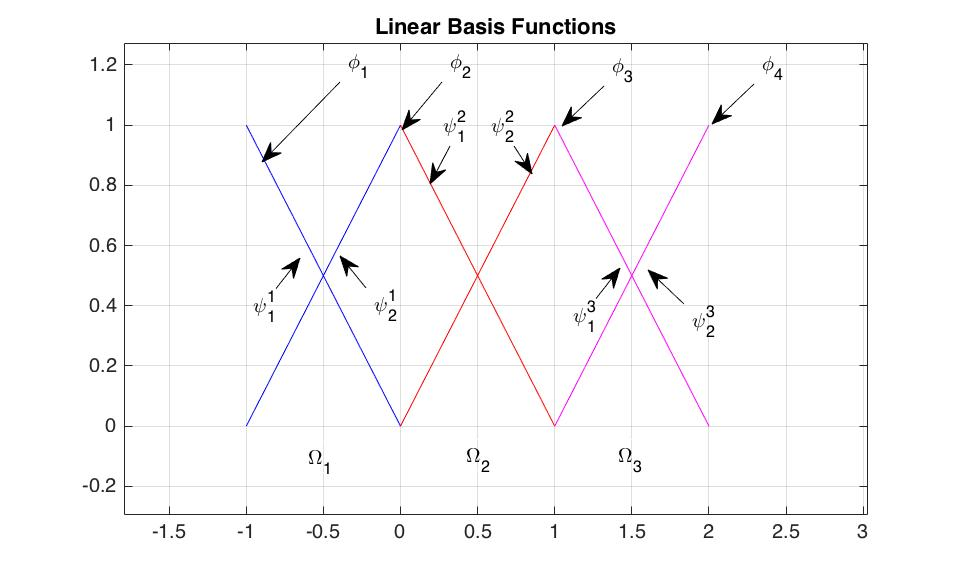
\includegraphics[scale = 0.4]{images/linearbasis.jpg}
		\caption{Basis Functions}
	\end{figure}
\end{center}
\pagebreak
\subsection{Assesmbly}
Upon adding the contributions of different element for any node $x_i$, we obtain the global stiffness matrix. This process is known as \textbf{Assembly} of the local siffness matrices. If $h_1, h_2, \dots, h_n$ are the element sizes, then the \textbf{global stiffness matrix A}  can easily be constructed as follows.
\begin{equation}
A = 
\begin{bmatrix}
\frac{1}{h_1} & -\frac{1}{h_1} & 0 & \dots & 0 & 0 & 0\\
-\frac{1}{h_1} & 	\frac{1}{h_1} + \frac{1}{h_2} & -\frac{1}{h_2} & \dots & 0 & 0 & 0\\
0 & 	-\frac{1}{h_2} & 	\frac{1}{h_2} + \frac{1}{h_3} & \dots & 0 & 0 & 0\\
\vdots & \vdots & \vdots & \vdots & \vdots & \vdots & \vdots\\
0 & 0 & 0 & \dots & -\frac{1}{h_{n-1}}  & \frac{1}{h_{n-1}} + \frac{1}{h_n} & 	-\frac{1}{h_n} \\
0 & 0 & 0 & \dots & 0  & -\frac{1}{h_n}  & \frac{1}{h_n} \\
\end{bmatrix} \label{assemA}
\end{equation}
and the \textbf{global load vector b} is,
\begin{equation}
b = 
\begin{Bmatrix}
\int_{0}^{h_1} f \psi_1^1 dx\\\\
\int_{0}^{h_1} f \psi_2^1 dx + \int_{h_1}^{h_2} f \psi_1^2 dx\\\\
\int_{h_1}^{h_2} f \psi_2^2 dx + \int_{h_2}^{h_3} f \psi_1^3 dx\\\\
\vdots\\\\
\int_{h_{n-2}}^{h_{n-1}} f \psi_2^{n-1} dx + \int_{h_{n-1}}^{h_n} f \psi_1^n dx\\\\
\int_{h_{n-1}}^{h_n} f \psi_2^n dx

\end{Bmatrix}\label{assemb}
\end{equation}
The next step is to apply the boundary conditions to the system $A \xi = b$ by setting the values accordingly in the Stiffness Matrix and Load Vector.\\


When we make the approximation by choosing $u_h$ from $V_h \subset V$, we introduce errors in the solution. If $u(x)$ denotes the exact solution and $u_h(x)$ denotes the Finite Element solution, we mention the following \textbf{error estimates} when a linear basis function is used. If $\lVert . \rVert_a$ denotes the energy norm, $\lVert . \rVert_\infty$ denotes the pointwise inifinity norm and $\lVert . \rVert_{H^m}$ denotes the $H^m$ norm we have the following error estimates
\begin{eqnarray}
\lVert u - u_h \rVert_a &\le& Ch \lVert u'' \rVert_\infty\\
\lVert u - u_h \rVert_{\infty} &\le& Ch^2 \lVert u'' \rVert_\infty \label{orderofconv}\\ 
\lVert u - u_h \rVert_{H^1} &\le& Ch \lVert u'' \rVert_\infty
\end{eqnarray}
Result \ref{orderofconv} shows that the Finite Element Method is second order accurate when linear basis is used.

\section{Numerical Examples}
\begin{example}
	Consider the following 2-Point Boundary Value Problem,
	\begin{eqnarray}
		-u'' = x(3+x)e^x, \quad 0<x<1\\
		u(0) = u(1) = 0
	\end{eqnarray}
	
		The exact solution is given by
		\begin{equation}
			u(x) = x(1-x)e^x
		\end{equation}
		
		We wish to find the solution to this problem using Finite Element Method.\\
		
		The weak form for the problem is given by \ref{weak1} with $f(x) = 1$ .\\
		
		 Assuming uniform grid spacing - $h$ while discretizing the domain into $n$ elements
		 \begin{eqnarray}
		 	 0&=&x_0 < x_2 < \dots < x_n = 1 \\
		 	 h &=& \frac{x_n - x_0}{n}\\
		 	 x_i &=& i \ h
		 \end{eqnarray}
		 
		  we have the finite dimensional weak form,
		 \begin{eqnarray}
		 	\text{Find} \; u_h \in V_h \subset V = H^1_0(0,1), \; \text{such that} \\
		 	\int_{0}^{1} u_h' v_h' \ dx = \int_{0}^{1} f v_h \ dx \quad \forall v_h \in V_h 	 	 
		 \end{eqnarray}	
		 
		 When we construct the element stiffness matrix, $K^e$, we get 
		 \begin{equation}
		 	K^e = \begin{bmatrix}
		 	\frac{1}{h} & -\frac{1}{h} \\
		 	-\frac{1}{h} & \frac{1}{h} 
		 	\end{bmatrix}
		 \end{equation}
		 
		 and after assembly (Ref. \ref{assemA}, \ref{assemb}) we obtain the system of linear equations.
		 \begin{equation}
		 	A \xi = b
		 \end{equation}
		 
		 and we solve the system of equations after accounting for the boundary conditions.	The solution plots for different number of elements are shown in Figure,\\
		 
		 \begin{figure}[h!]
		 		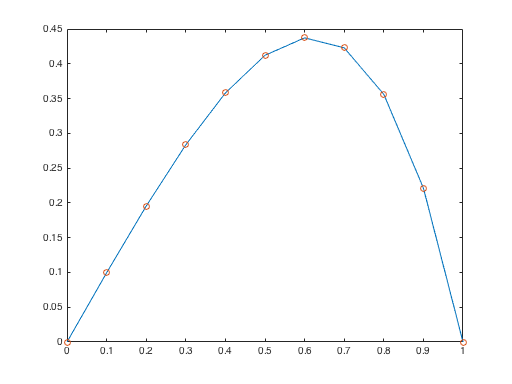
\includegraphics[scale = 0.8]{images/firstex.png}
		 		\caption{$Numerical Solution$}
		 \end{figure}
		 
		The infinity norm of the error in the Finite Element Solution was found out to be in the order of $\approx 10^{-16}$ which is very close to the machine error $\approx 2.2 \times 10^{-16}$
		

\end{example}

\begin{example}
		Consider the following 2-Point Boundary Value Problem,
		\begin{eqnarray}
		-u'' + u &=& 12x + 3x^2 - 2x^3 - 6, \quad 0<x<1\\
		u(0) &=& 0\\
		u'(1) &=& 0
		\end{eqnarray}
		
		The weak form for this problem is given by,
		\begin{eqnarray}\nonumber
		\text{Find} \; u_h \in V_h \subset V = \{u \ | \ u \in H^1(0,1), \ u(0) = 0\}, \; \text{such that} \\\nonumber
		- u_h'v_h \Big|_0^1 + \int_{0}^{1} (u_h' v_h' + u_h v_h) \ dx = \int_{0}^{1} f v_h \ dx \qquad &\forall v_h \in V_h&	\\
		\implies \int_{0}^{1} (u_h' v_h' + u_h v_h) \ dx = \int_{0}^{1} f v_h \ dx  + u_h'(1)v_h(1)\qquad &\forall v_h \in V_h&\\
		\implies \int_{0}^{1} (u_h' v_h' + u_h v_h) \ dx = \int_{0}^{1} f v_h \ dx  \qquad &\forall v_h \in V_h&
		\end{eqnarray}	
		
		The Neumann Boundary Condition is accounted in the assembled RHS by adding the value of $u'(1)$ in the last entry of $b$.\\
		
		Hence the final system of equations become,
		\begin{equation}
			A \xi = b + \vec{f_n}
		\end{equation}
		
The order of convergence observed for different elements are tabulated below,\\
		\begin{center}
			\begin{tabular}{|c|c|}
				\hline
				Element Type & Order of convergence observed\\
				\hline
				Linear & $\approx 2$\\
				Quadratic & $\approx 4$\\
				Cubic & $\approx 5$\\
				\hline						
			\end{tabular}
		\end{center}
		\begin{figure}[h!]
						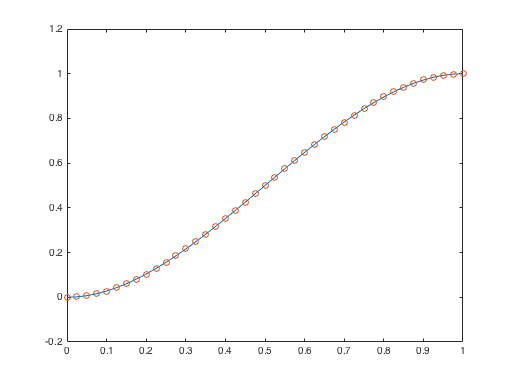
\includegraphics[scale = 0.8]{images/secondex.png}
						\caption{$n = 40$}	
		\end{figure}
\end{example}

\begin{example}
	Consider the following 2-Point Boundary Value Problem,
	\begin{eqnarray}
	-u'' + u &=& x^2+x-2, \quad 0<x<1\\
	u(0) &=& 0\\
	u(1)+u'(1) &=& 5
	\end{eqnarray}
	
	The weak form for this problem is given by,
	\begin{eqnarray}\nonumber
	\text{Find} \; u_h \in V_h \subset V = \{u \ | \ u \in H^1(0,1), \ u(0) = 0\}, \; \text{such that} \\\nonumber
	- u_h'v_h \Big|_0^1 + \int_{0}^{1} (u_h' v_h' + u_h v_h) \ dx = \int_{0}^{1} f v_h \ dx \qquad &\forall v_h \in V_h&	\\
	\implies \int_{0}^{1} (u_h' v_h' + u_h v_h) \ dx = \int_{0}^{1} f v_h \ dx  + u_h'(1)v_h(1)\qquad &\forall v_h \in V_h&\\
	\implies \int_{0}^{1} (u_h' v_h' + u_h v_h) \ dx = \int_{0}^{1} f v_h \ dx  + (5 - u_h(1)) \ v_h(1)\qquad &\forall v_h \in V_h&
	\end{eqnarray}	
	The Robin Boundary Condition is accounted in the assembled R.H.S by adding the value of $u'(1)+u(1) = 5$ in the last entry of $b$, and since $u_h(1)$ appears in the R.H.S, the value must be accounted for in the assembled global stiffness matrix.\\
	
	Hence the final system of equations become,
	\begin{equation}
		\begin{bmatrix}
		A_{11} & A_{12} & \dots & A_{1n}\\
		\vdots & \vdots & \vdots & \vdots\\
		A_{n1} & A_{n2} & \dots & A_{nn}
		\end{bmatrix} 
		\begin{Bmatrix}
		\xi_1\\
		\vdots\\
		\xi_n
		\end{Bmatrix} = 
		\begin{Bmatrix}
		b_1\\
		\vdots\\
		b_n
		\end{Bmatrix} +
		\begin{Bmatrix}
		0\\
		\vdots\\
		5 - \xi_n
		\end{Bmatrix}
	\end{equation}
	which in-turn becomes,
	\begin{equation}
		\begin{bmatrix}
		A_{11} & A_{12} & \dots & A_{1n}\\
		\vdots & \vdots & \vdots & \vdots\\
		A_{n1} & A_{n2} & \dots & A_{nn}+1
		\end{bmatrix} 
		\begin{Bmatrix}
		\xi_1\\
		\vdots\\
		\xi_n
		\end{Bmatrix} = 
		\begin{Bmatrix}
		b_1\\
		\vdots\\
		b_n
		\end{Bmatrix} +
		\begin{Bmatrix}
		0\\
		\vdots\\
		5
		\end{Bmatrix}
	\end{equation}
	
	The plots showing the solution curves for a Cubic Element is shown in Figure \ref{fig5}. The error in the Finite Element solution is in the order of $\approx 10^{-13}$
	
	\begin{figure}[h!]
			\begin{subfigure}{0.5\textwidth}
				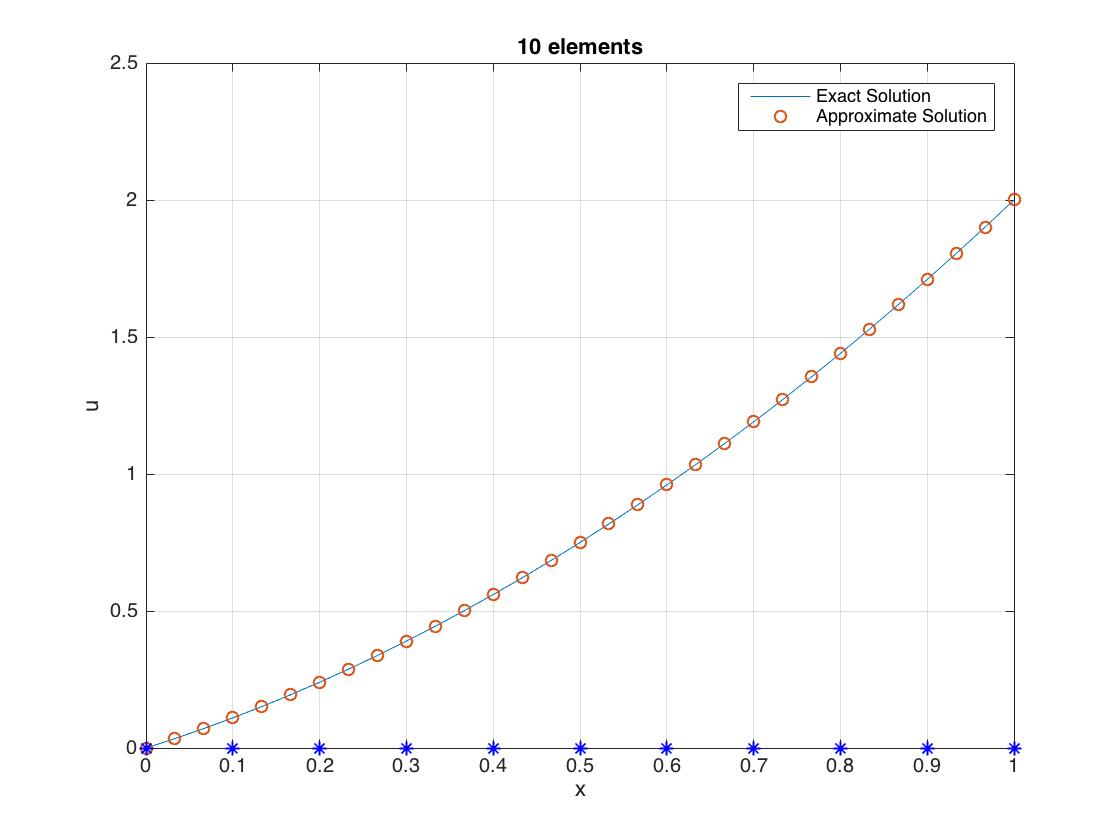
\includegraphics[scale = 0.2]{images/ex3/cubic10.jpg}
				\caption{$n = 10$}	
			\end{subfigure}
			\begin{subfigure}{0.5\textwidth}
				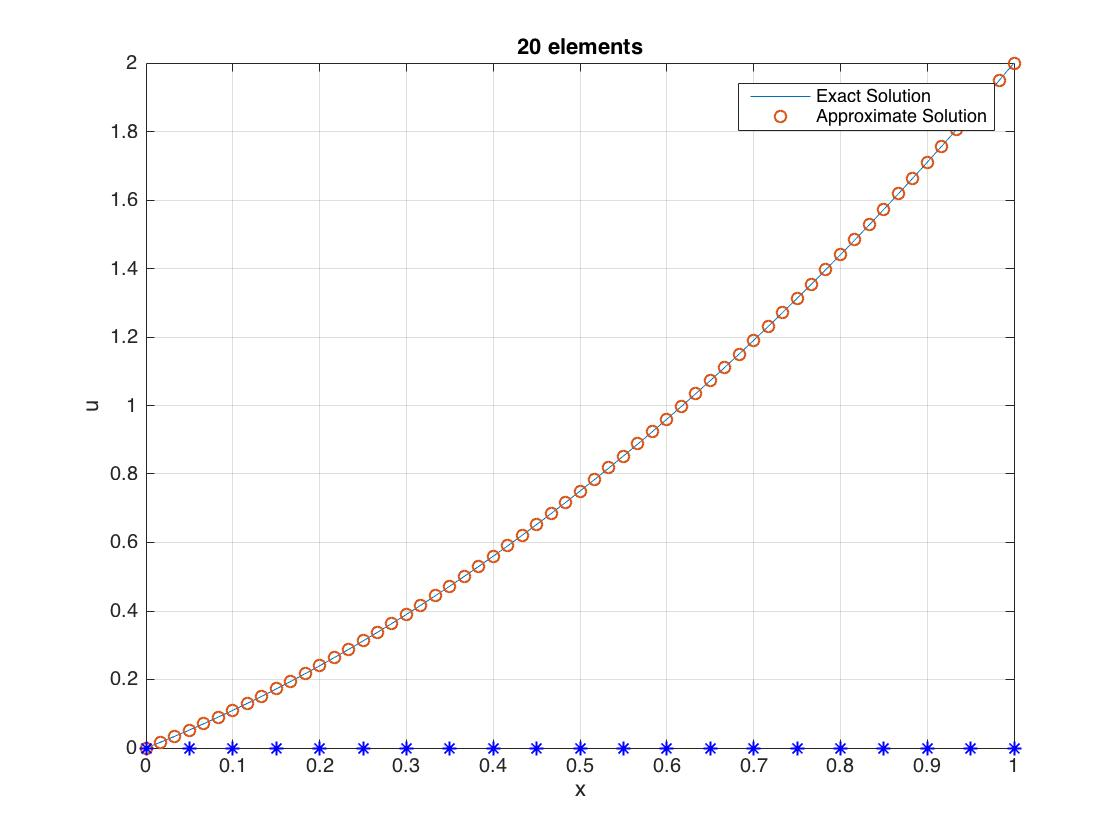
\includegraphics[scale = 0.2]{images/ex3/cubic.jpg}
				\caption{$n = 20$}	
			\end{subfigure}
			\caption{Solution plots using cubic elements - Example 2.3}
			\label{fig5}		
	\end{figure}
\end{example}

\section{Non-Linear Problem}
Next we consider solving a non-linear problem using Finite Element Method. We obtain a non-linear system of equations,
\begin{equation}
	K(U) \ U = F \quad \text{or} \quad K U = F(U) 
\end{equation}
So, we use the \textbf{Newton Raphson} iterations to solve the system of equations. The procedure is to first construct the system of equations at the element level,
\begin{equation}
	K^e(u^e) \ u^e = f^e
\end{equation}
and compute the elemental Jacobian Matrix $J^e$. Next we assemble the elemental Jacobian and the elemental load vector to the global level $J$ and $F$ and use Newton Raphson Iterations,
\begin{enumerate}
	\item Define $error = 100$ and tolerance $tol = 10^{-10}$ and Initial Guess $U_{old}$.
	\item Compute elemental Jacobian Matrix and Load Vector $J^e$ and $F^e$
	\item while $error > tol$:
	\begin{eqnarray}\nonumber
		&\text{Assemble: }& \quad J^e \ \text{and} \ F^e \implies J \ and \ F\\\nonumber
		&\text{Apply Boundary Conditions}&\\\nonumber
		& \text{Newton Raphson Iteration:}& \quad U_{new} = U_{old} - (J^{-1} F)(U_{old})\\\nonumber
		& \text{Set} & \quad error = \lVert U_{new} - U_{old} \rVert\\\nonumber
		& \text{Do} & \quad U_{old} = U_{new}
	\end{eqnarray}
\end{enumerate}

\begin{example}
	Consider the following 2-Point Boundary Value Problem,
	\begin{eqnarray}
	-u'' + (u')^3 &=& 0, \quad 0<x<1\\
	(u+u')(0) &=& 3/\sqrt{2}\\
	u'(1) &=& 0.5
	\end{eqnarray}
	
	The exact and the approximate solution are shown in Figure \ref{fig6}. The order of convergence is found to be $2$, when linear basis functions are used.
	\begin{figure}[h]
		\begin{subfigure}{0.5\textwidth}
			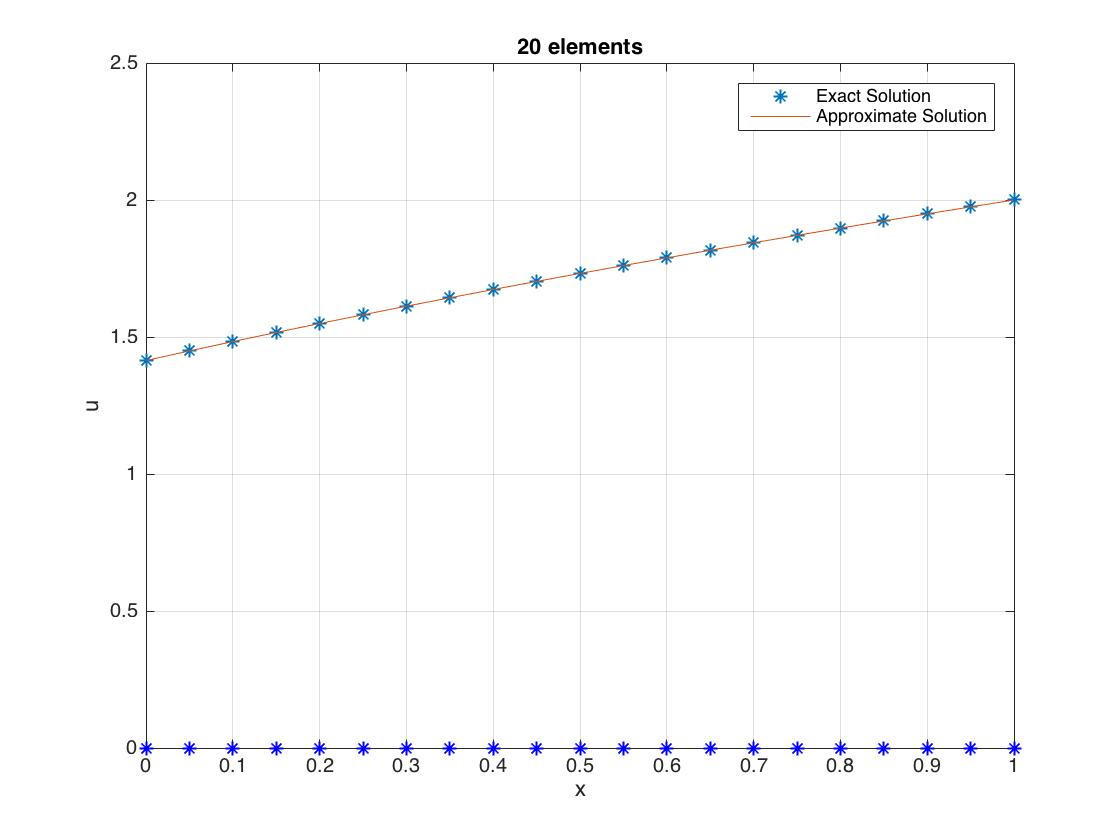
\includegraphics[scale = 0.2]{images/ex4/nonlinear.jpg}
			\caption{$n=20$}
		\end{subfigure}	
	\begin{subfigure}{0.5\textwidth}
		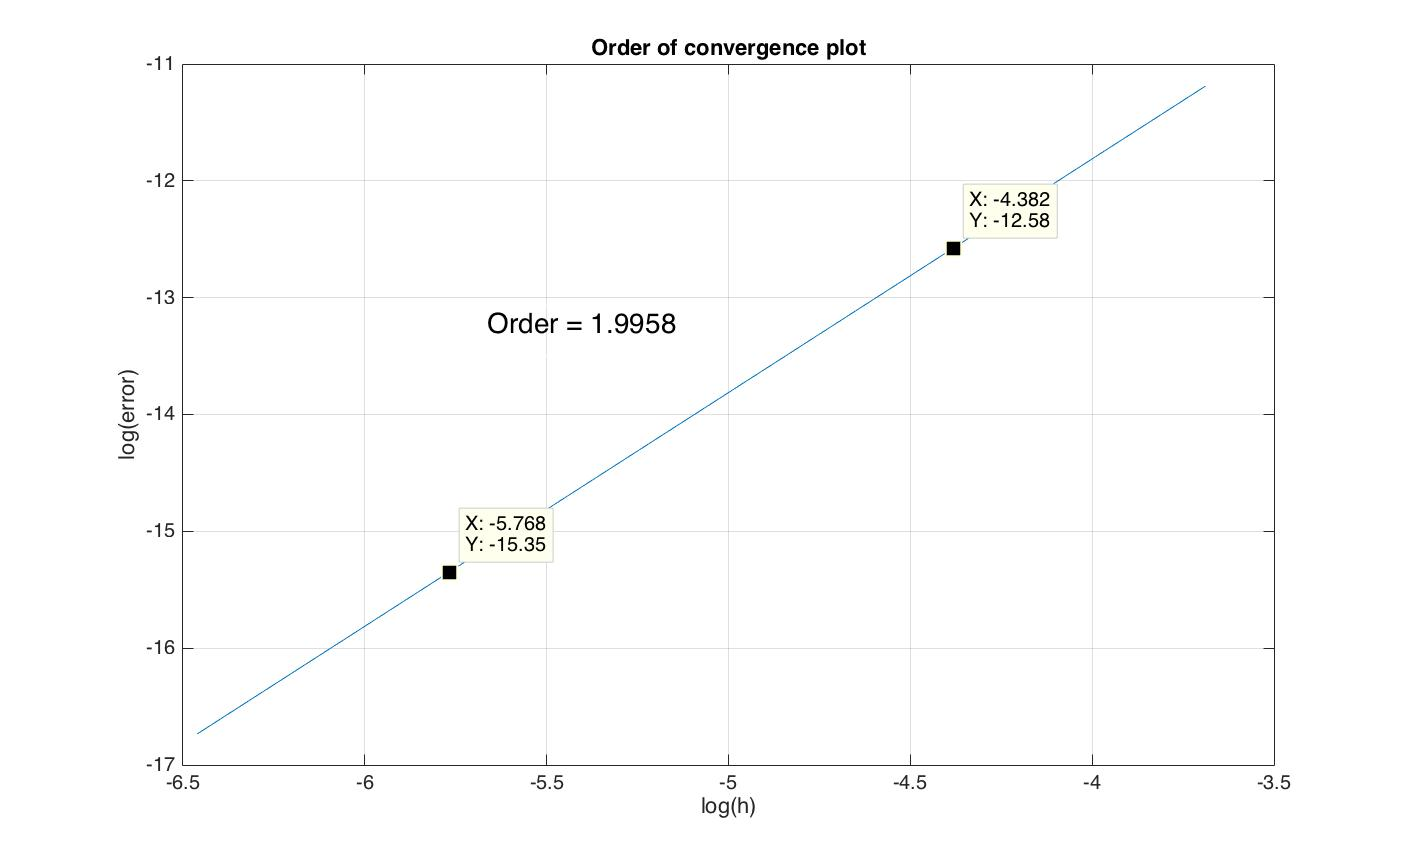
\includegraphics[scale = 0.2]{images/ex4/non_order.jpg}
		\caption{Order of convergence $\approx 2$}
	\end{subfigure}
	\caption{Non Linear Problem - Example 2.4}	
	\label{fig6}
	\end{figure}
\end{example}
